\documentclass[a4paper,11pt]{article}

\usepackage[utf8]{inputenc}

\usepackage{graphicx}
\usepackage{caption}
\usepackage{subcaption}

\usepackage{pgfplots}
\pgfplotsset{compat=1.18} 

\usepackage{minted}
\usepackage{siunitx}
\usepackage{tikz}

\usetikzlibrary{positioning}

\usetikzlibrary{arrows.meta,positioning,calc}
\usepackage{booktabs}
\usepgfplotslibrary{groupplots}

\begin{document}

\title{
    \textbf{A heap or priority queue in C}
}
\author{Mo Wang}
\date{Spring 2026}

\maketitle

\section*{Introduction}
This report examines different priority-queue designs from simple lists to heaps, highlighting gradual performance progression. It begins from the two list-based priority queues that trades between $O(1)$ enqueue for $O(n)$ dequeue (unsorted insertion) and vice versa (sorted insertion). As an intermediate step, a BST offers average $O(\log n)$ operations but can skew under realistic workloads, degrading into $O(n)$ complexity. To ensure predictable efficiency, a heap is implemented as a linked tree that balances by subtree size, and finally as a compact implicit array whose contiguous structure improves cache locality. Benchmarks confirm the pattern: the final array heap delivers the most optimal behavior for practical usage while the linked‑tree heap is close and stable. On the other hand, list and unbalanced BST approaches exhibit clear performance limitations.

\section*{List Priority Queue}
\subsection*{Data structure}

A list priority queue can be built using a resizable array list. The control block data structure consists of the pointer to the first element of the array, as well as number of elements currently in queue and its maximum capacity, which are required for insertion and deletion operations.

\begin{minted}{C}
typedef struct list_pq1{
    int *arr;           // Dynamic array to store elements
    unsigned int top;   // Number of elements currently in queue
    unsigned int cap;   // Maximum capacity
} list_pq1;
\end{minted}

\subsection*{Implementations}

There are two different implementations of list priority queues using arrays.

The first implementation is unsorted insertion approach where an element is appended at the end of the array during enqueue. However, the dequeue operation requires searching the element with highest priority and removing it.

Another implementation is sorted insertion approach and involves inserting an element into an array at the correct position according to its priority during the enqueue operation. Dequeueing becomes straightforward, as it can be performed by simply removing the last element of the array with the highest priority.

In both approaches, smaller integers have higher priority.

\subsection*{List Priority Queue 1}
\subsubsection*{Enqueue}

During enqueue operation, an element is simply attached to the tail of the array. However, when the array is full, the operation fails and returns false to indicate the failure. The time complexity is constant $O(1)$ since no sorting or searching is required.

\begin{minted}{C}
bool list_pq1_enqueue(list_pq1 *nh, int val){
    if (!nh || nh->top >= nh->cap) return false;  // Check if full
    nh->arr[nh->top++] = val;  // Add element and increment size
    return true;
}
\end{minted}

\subsubsection*{Dequeue}
The dequeue operation removes the element with the highest priority from the array. Since the array is unsorted, it requires a linear search to find the element with highest priority, which is the minimum element in this case. Once the it is found, it is removed, while all subsequent elements are subsequently shifted to fill the gap. As a result, the time complexity is $O(n)$.

\begin{minted}{C}
bool list_pq1_dequeue(list_pq1 *nh, int *res_ptr){
    if (!nh || nh->top == 0 || !res_ptr) return false;  // Check if empty

    // Step 1: Linear search to find minimum element - O(n)
    unsigned int min_index = 0;
    int min = nh->arr[0];
    for (unsigned int i = 1; i < nh->top; i++){
        if (nh->arr[i] < min){
            min = nh->arr[i];
            min_index = i;  // Track position of minimum
        }
    }
    
    *res_ptr = min;  // Return the minimum value
    
    // Step 2: Shift all elements after minimum to the left - O(n)
    for (unsigned int i = min_index; i < nh->top - 1; i++){
        nh->arr[i] = nh->arr[i + 1];
    }
    nh->top--;  // Decrease size
    return true;
}
\end{minted}

\subsection*{List Priority Queue 2}
\subsubsection*{Enqueue}
In sorted insertion approach, during enqueue operation, a desired empty place needs to be found while smaller elements to the position are subsequently shifted to the right. Afterwards, the element can be placed into the gap to maintain the descending sorted order of the array. Therefore, the time complexity is linear $O(n)$, since the full array is traversed.

\begin{minted}{C}
bool list_pq2_enqueue(list_pq2 *nh, int val){    
    if (!nh || nh->top >= nh->cap) return false;  // Check if full
    
    // Find insertion position by shifting smaller elements right
    int i = (int) nh->top-1;
    while (i >= 0 && nh->arr[i] < val){
        nh->arr[i+1] = nh->arr[i];  // Shift element right
        i--;
    }
    nh->arr[i+1] = val;  // Insert at correct sorted position
    nh->top++;           // Increment size
    return true;
}
\end{minted}

\subsubsection*{Dequeue}

The dequeue operation removes the element at the tail of the array, which is always the minimum value with highest priority, since the array is already sorted in a descending order. This yields constant time complexity $O(1)$.

\begin{minted}{C}
bool list_pq2_dequeue(list_pq2 *nh, int *res_ptr){
    if (!nh || nh->top == 0 || !res_ptr) return false;  // Check if empty
    *res_ptr = nh->arr[--nh->top];  // Return and remove last element (minimum)
    return true;
}
\end{minted}

\subsection*{benchmark comparison (LPQ1 vs LPQ2)}

The given time complexity can be conformed by benchmark comparisons. Enqueue operation in list priority queue 1, an unsorted insertion approach, has a constant time complexity $O(1)$, while dequeue operation exhibits a growing linear time complexity $O(n)$ with orders of magnitudes higher execution time compared enqueue operation, which can be observed in Table~\ref{tab:pq1-pq2} and Figure~\ref{fig:pq1-pq2-comparison}. On the other hand, in Table~\ref{tab:pq1-pq2} and Figure~\ref{fig:pq1-pq2-comparison}, the time complexities for list priority queue 2, a sorted insertion approach, are swapped for both operations compared to the first implementation. Enqueue operation yields constant time complexity $O(1)$, orders of magnitude below dequeue operation with linear time complexity $O(n)$.

\begin{table}[h!]
\centering
\begin{tabular}{rccccccc}
\toprule
\textbf{Size}
    & 1024 & 2048 & 4096 & 8192 & 16384 & 32768 & 65536 \\
\midrule
\textbf{LPQ1 Enq (ns)}
    & 17.86 & 19.16 & 25.89 & 26.13 & 28.36 & 37.47 & 30.01 \\
\textbf{LPQ1 Deq (ns)}
    & 2938.77 & 5288.57 & 10601.14 & 22247.20 & 44382.82 & 88949.90 & 173798.53 \\
\hline
\textbf{LPQ2 Enq (ns)}
    & 842.52 & 1604.57 & 3220.07 & 6686.55 & 13323.77 & 26408.27 & 52486.53 \\
\textbf{LPQ2 Deq (ns)}
    & 15.03 & 15.05 & 17.05 & 17.07 & 22.65 & 22.91 & 26.91 \\
\bottomrule
\end{tabular}
\caption{LPQ1 ($O(1)$ enqueue, $O(n)$ dequeue) vs.\ LPQ2 ($O(n)$ enqueue, $O(1)$ dequeue).}
\label{tab:pq1-pq2}
\end{table}

\begin{figure}[h!]
\centering
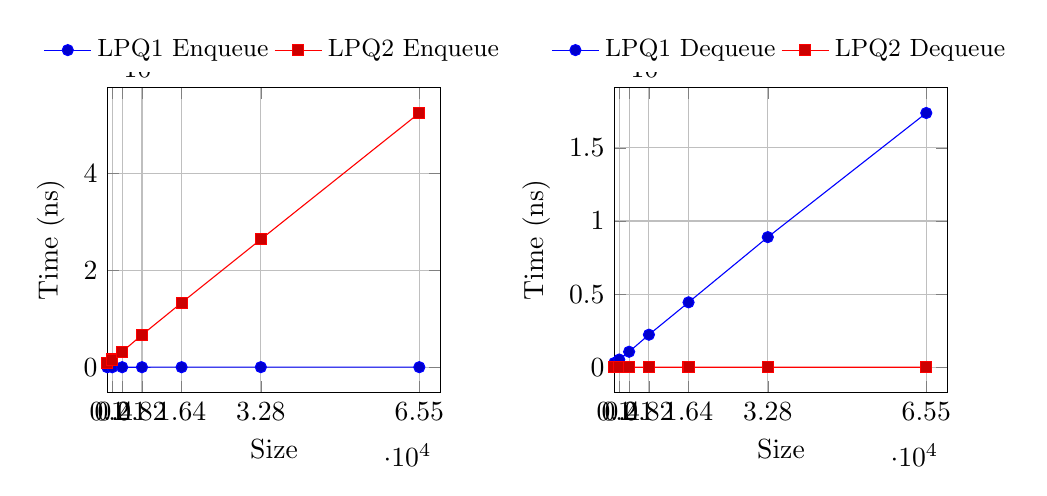
\begin{tikzpicture}
\begin{groupplot}[
  group style={group size=2 by 1, horizontal sep=2.2cm},
  width=0.48\textwidth,
  height=0.45\textwidth,
  xlabel={Size},
  % ymode=log,
  ylabel={Time (ns)},
  xmin=1000, xmax=70000,
  xtick={1024,2048,4096,8192,16384,32768,65536},
  xticklabel style={/pgf/number format/fixed},
  legend style={font=\small, at={(0.5,1.05)}, anchor=south, draw=none, legend columns=2},
  grid=both
]

% ---------- LEFT: ENQUEUE ----------
\nextgroupplot[
  title={Enqueue Time Comparison},
]
% PQ1 Enqueue
\addplot+[mark=*] coordinates {
  (1024,17.86) (2048,19.16) (4096,25.89) (8192,26.13)
  (16384,28.36) (32768,37.47) (65536,30.01)
};
\addlegendentry{LPQ1 Enqueue};

% PQ2 Enqueue
\addplot+[mark=square*] coordinates {
  (1024,842.52) (2048,1604.57) (4096,3220.07) (8192,6686.55)
  (16384,13323.77) (32768,26408.27) (65536,52486.53)
};
\addlegendentry{LPQ2 Enqueue};

% ---------- RIGHT: DEQUEUE ----------
\nextgroupplot[
  title={Dequeue Time Comparison},
]
% PQ1 Dequeue
\addplot+[mark=*] coordinates {
  (1024,2938.77) (2048,5288.57) (4096,10601.14) (8192,22247.20)
  (16384,44382.82) (32768,88949.90) (65536,173798.53)
};
\addlegendentry{LPQ1 Dequeue};

% PQ2 Dequeue
\addplot+[mark=square*] coordinates {
  (1024,15.03) (2048,15.05) (4096,17.05) (8192,17.07)
  (16384,22.65) (32768,22.91) (65536,26.91)
};
\addlegendentry{LPQ2 Dequeue};

\end{groupplot}
\end{tikzpicture}
\caption{Comparison of LPQ1 ($O(1)$ enqueue, $O(n)$ dequeue) and LPQ2 ($O(n)$ enqueue, $O(1)$ dequeue) across sizes. Logarithmic y-axis highlights expected trade-offs.}
\label{fig:pq1-pq2-comparison}
\end{figure}


\section*{Intermediate solution: BST}

In order to improve performance of a priority queue from constant time complexity in either enqueue or dequeue operation, a binary search tree (BST) can be used providing average-case logarithmic time complexity for both enqueue and dequeue operations. Since a BST always maintain a sorted order for in-order traversal, the smallest element always resides in the left-most node while the largest always in right-most node. This allows dequeuing the smallest element with highest priority to be efficiently performed by removing the leftmost node. However, the tree can be right-skewed after multiple enqueue and dequeue operations, degenerating into linear time complexity $O(n)$.

\subsection*{Data structure}

The data structure of BST heap is same to BST tree. There are two structures: a node structure for holding a value and two pointer addresses to its left and right subtrees as well as a BST tree control block for holding the root node pointer address.

\begin{minted}{C}
typedef struct bst_node {
    int value;
    struct bst_node *left;   // Left subtree: values < current
    struct bst_node *right;  // Right subtree: values > current
} bst_node;

typedef struct bst_tree {
    bst_node *root;
} bst_tree;
\end{minted}

\subsection*{Enqueue}
The enqueue operation inserts an element into the BST tree while maintaining its order. It can be implemented recursively by checking the insertion value with the current node value. If the value matches the node value, it already exists and does nothing. Otherwise, depending on the insertion value being greater or less than current node value, respective node will be proceeded, until leaf node is reached where the value is attached. This yields logarithmic time complexity in best case $O(\log n)$

\begin{minted}{C}
static bst_node* add_node(bst_node *nd, int value){
    if (nd == NULL){
        return construct_bst_node(value);  // Create new leaf node
    }
    // Recursively insert based on comparison
    if (value < nd->value){
        nd->left = add_node(nd->left, value);   // Go left for smaller values
    }
    else if (value > nd->value){
        nd->right = add_node(nd->right, value); // Go right for larger values
    }
    // If value == nd->value, do nothing (no duplicates)
    return nd;
}
\end{minted}

The recursive logic is implemented in the function \texttt{add\_node}, whereas the initial value is handled by the function \texttt{bst\_heap\_enqueue}.

\begin{minted}{c}
bool bst_heap_enqueue(bst_tree *tr, int value){
    if (tr == NULL) return false;
    tr->root = add_node(tr->root, value);
    return true;
}
\end{minted}

\subsection*{Dequeue}

The dequeue operation can be implemented by removing the minimum element with the highest priority, which is the leftmost node of the BST tree. The algorithm turns to the left subbranch until the leftmost leaf node is reached, while tracking its parent node. Afterwards, the leftmost node is removed, while its right node is promoted to its position, if it exists. The time complexity is proportional to the height of the tree, which yields logarithmic time complexity $O(\log n)$ in best case.

\begin{minted}{C}
bool bst_heap_dequeue(bst_tree *tr, int* res_ptr) {
    if (tr == NULL || tr->root == NULL) {
        return false;  // Empty tree
    }
    bst_node *parent = NULL;
    bst_node *current = tr->root;

    // Traverse to leftmost node (minimum in BST)
    // This is the node with no left child
    while (current->left != NULL) {
        parent = current;
        current = current->left;
    }

    *res_ptr = current->value;  // Return minimum value

    // Remove the minimum node and reconnect tree
    if (parent == NULL) {
        // Minimum is root (no left child at root)
        tr->root = current->right;  // Root becomes its right subtree
    }
    else {
        // Minimum is not root
        parent->left = current->right;  // Bypass current node
    }

    free(current);  // Free the removed node
    return true;
}
\end{minted}

\subsection*{Benchmark and analysis}

However, since each dequeue operation removes the left-most node, the BST tree can becomes right-skewed unbalanced after multiple enqueue and dequeue operations when it is used as a priority queue. Considering that the BST is not self-balanced, the tree can degenerate into a right-skewed chain where both enqueue and dequeue operation degrades from logarithmic time complexity $O(\log n)$ into linear time complexity $O(n)$. Additionally, BST degeneration is inevitable, since enqueue operation does not always compensate for the leftmost removed element.

A BST does not enforce heap structure; instead, ordering is by in‑order traversal (left - root - right). Removing the minimum element always means “take the leftmost node”. This structure can become skewed (unbalanced) when used as a priority queue.

In both Table~\ref{tab:bst-pq-transposed} and Figure~\ref{fig:bst-pq-fitted}, the behavior of an initial logarithmic time complexity and a linear time complexity due to skewed BST can be observed from the execution time from BST tree benchmark. The benchmark consists of a series of enqueue operation as well a series of dequeue operation, which yields linear time complexity for large amount of repeated enqueue and dequeue operations.

% =========================
% TABLE
% =========================
\begin{table}[h]
\centering
\begin{tabular}{l|ccccccc}
\textbf{Repeats}
    & 1024 & 2048 & 4096 & 8192 & 16384 & 32768 & 65536 \\
\hline
\textbf{Enqueue (ns/op)}
    & 90.29 & 113.06 & 127.70 & 137.38 & 162.67 & 253.23 & 439.27 \\
\textbf{Dequeue (ns/op)}
    & 52.21 & 59.76 & 63.15 & 57.75 & 92.80 & 88.97 & 110.56 \\
\end{tabular}
\caption{Benchmark results for a BST-based priority queue}
\label{tab:bst-pq-transposed}
\end{table}

% =========================
% FIGURE (PGFPlots)
% Updated fitted lines from new data
% Requires in preamble:
%   \usepackage{pgfplots}
%   \pgfplotsset{compat=1.18}
% =========================
\begin{figure}[h]
\centering
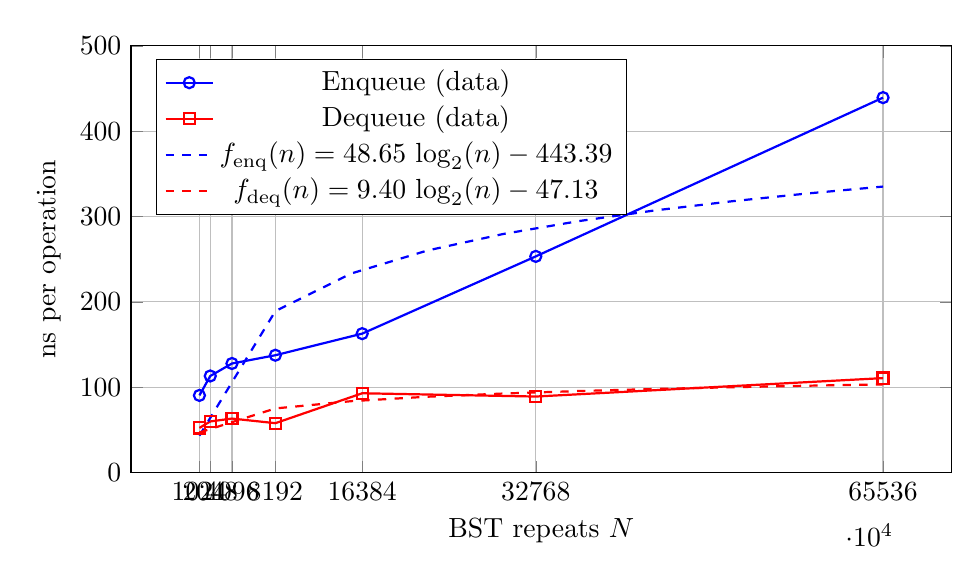
\begin{tikzpicture}
\begin{axis}[
    width=12cm,
    height=7cm,
    xlabel={BST repeats $N$},
    ylabel={ns per operation},
    xtick={1024,2048,4096,8192,16384,32768,65536},
    xticklabels={1024,2048,4096,8192,16384,32768,65536},
    legend pos=north west,
    grid=both,
    ymin=0, ymax=500
]

% ----------------------
% Enqueue data (points)
% ----------------------
\addplot[
    color=blue,
    mark=o,
    thick
]
coordinates {
    (1024,90.29)
    (2048,113.06)
    (4096,127.70)
    (8192,137.38)
    (16384,162.67)
    (32768,253.23)
    (65536,439.27)
};
\addlegendentry{Enqueue (data)}

% ----------------------
% Dequeue data (points)
% ----------------------
\addplot[
    color=red,
    mark=square,
    thick
]
coordinates {
    (1024,52.21)
    (2048,59.76)
    (4096,63.15)
    (8192,57.75)
    (16384,92.80)
    (32768,88.97)
    (65536,110.56)
};
\addlegendentry{Dequeue (data)}

% ----------------------
% Fitted line for Enqueue
% f_enq(n) = 48.6518 * log2(n) - 443.3875
% ----------------------
\addplot[
    color=blue,
    dashed,
    thick,
    domain=1024:65536,
    samples=10
]
{48.6517857142858 * log2(x) - 443.3875};
\addlegendentry{$f_{\mathrm{enq}}(n)=48.65\,\log_2(n)-443.39$}

% ----------------------
% Fitted line for Dequeue
% f_deq(n) = 9.3971 * log2(n) - 47.1343
% ----------------------
\addplot[
    color=red,
    dashed,
    thick,
    domain=1024:65536,
    samples=10
]
{9.39714285714288 * log2(x) - 47.134285714286};
\addlegendentry{$f_{\mathrm{deq}}(n)=9.40\,\log_2(n)-47.13$}

\end{axis}
\end{tikzpicture}
\caption{BST priority queue performance with algebraic fitted curves}
\label{fig:bst-pq-fitted}
\end{figure}

\subsection*{Motivation for heap}
A BST tree orders keys by in-order traversal but does not enforce a complete-tree shape, so typical insertion/removal patterns can skew the tree and degrade operations to $O(n)$. The time complexities are described in Table~\ref{tab:op-complexity}. However, implementing a self-balancing BST tree for a priority queue, such as AVL, red-black trees, or B+ trees, can guarantee logarithmic time complexity $O(\log n)$ but causes large performance overhead.

So, a new data structure (heap) is designed to enforce the heap-order property on a complete tree, giving $O(1)$ finding the minimum value and $O(\log n)$ insertion and deletion of minimum regardless of key order.

% So the BST structure is not suitable as a heap unless a self‑balancing BST (AVL, red‑black) is applied, but that would be much complicated and expensive solution.a BST is not designed to guarantee for a priority queue.

\begin{table}[h]
\centering
\begin{tabular}{lcc}
\hline
\textbf{Operation} & \textbf{Best} & \textbf{Worst} \\
\hline
Insert & $O(\log n)$ & \textbf{$O(n)$} \\
Remove & $O(\log n)$ & \textbf{$O(n)$} \\
\hline
\end{tabular}
\caption{Asymptotic time complexity for operations.}
\label{tab:op-complexity}
\end{table}

\section*{Heap implemented by linked tree}

A heap takes form in a binary tree structure, but unlike a BST tree, a node value must be smaller than its left and right child. However, there is no inherit relationship between the two children. As a result, the data structure for a heap in C code is the same as the BST tree, which is previously shown.

\subsection*{Peek (Find the smallest node in heap)}

A peek operation can be simply done by retrieving the minimum value, which sits in the root node which is guaranteed to hold the smallest value of the heap due to its invariants. As a result, the time complexity is constant $O(1)$.

\begin{minted}{C}
bool tree_heap_peek(heap *hp, int *res_ptr) {
    if (!hp->root)  return false;  // Empty heap
    *res_ptr = hp->root->value;  // Root always contains minimum
    return true;
}
\end{minted}

\subsection*{Enqueue (Insert a node in heap)}

Enqueue operation involves inserting a node into the heap. Whenever a new value is inserted into a subtree, it is compared with the top node of the subtree. If the new value is smaller, the values are swapped and the larger one is recursively pushed down into one of the child subtrees. The process continues until the bottom of the heap is reached, so its value is pushed down into one of the two subbranches recursively. When the bottom of the heap is reached, the value will be attached. The function also holds a pointer address to a boolean value, indicating either successful or failed operation (malloc failure).

\begin{minted}{C}
node *insert_node(node *nd, int value, bool* status_ptr) {
    if (nd == NULL) {
        node *new_node = create_node(value);
        if (!new_node) *status_ptr = false;
        return new_node;
    }

    // Maintain min-heap property: if new value smaller, swap with current
    // Push larger value down the tree
    if (value < nd->value) {
        int tmp = nd->value;
        nd->value = value;
        value = tmp;  // Continue inserting the larger value
    }

    // Insert into subtree with fewer nodes to keep tree balanced
    // This ensures O(log n) height
    if (get_size(nd->left) <= get_size(nd->right))
        nd->left = insert_node(nd->left, value, status_ptr);
    else
        nd->right = insert_node(nd->right, value, status_ptr);

    // Update size after insertion
    nd->size = 1 + get_size(nd->left) + get_size(nd->right);
    return nd;
}

bool tree_heap_enqueue(heap *hp, int value) {
    bool result = true;
    hp->root = insert_node(hp->root, value, &result);
    return result;
}
\end{minted}

\subsection*{Dequeue (Remove a node in heap)}

Removing the minimum element from the linked-tree heap is done by extracting the root, which always holds the smallest value. The removal is carried out by recursively promoting the smallest child up the tree: if both children exist, the child with the smaller value is swapped with the current node; if only one child is present, that child is promoted instead. This process continues until a leaf node is reached, at which point the node is freed. After each recursive step, the \texttt{size} field is updated to maintain accurate subtree counts. The wrapper function texttt{tree\_heap\_dequeue} simply stores the root value and replaces the root with the result of the recursive \texttt{remove\_node} call, ensuring that the heap property is preserved throughout the deletion operation.

\begin{minted}{C}
node *remove_node(node *root) {
    if (!root) return NULL;

    // Leaf node: simply remove it
    if (!root->left && !root->right) {
        free(root);
        return NULL;
    }

    // Promote smallest child to maintain heap property
    // This bubbles up the minimum from children
    if (root->left && root->right) {
        // Both children exist: choose smaller one
        if (root->left->value < root->right->value) {
            swap_node_values(root, root->left);
            root->left = remove_node(root->left);  // Recursively remove from left
        } else {
            swap_node_values(root, root->right);
            root->right = remove_node(root->right);  // Recursively remove from right
        }
    }
    else if (root->left) {
        // Only left child exists
        swap_node_values(root, root->left);
        root->left = remove_node(root->left);
    }
    else if (root->right) {
        // Only right child exists
        swap_node_values(root, root->right);
        root->right = remove_node(root->right);
    }

    // Update size after removal
    root->size = 1 + get_size(root->left) + get_size(root->right);
    return root;
}

bool tree_heap_dequeue(heap *hp, int *res_ptr) {
    if (!hp->root) {
        return false;
    }
    *res_ptr = hp->root->value;
    hp->root = remove_node(hp->root);
    return true;
}
\end{minted}

\subsection*{Balancing the tree}

To ensure that the linked-tree heap remains balanced, each node stores a \texttt{size} field in the data structure representing the total number of elements in its subtree. 

\begin{minted}{C}
typedef struct node {
    int value;
    int size;              // number of nodes in subtree (for balancing)
    struct node *left;
    struct node *right;
} node;
\end{minted}

During insertion, the algorithm compares the sizes of the left and right subtrees and always descends into the branch with the smaller size. This strategy guarantees that new nodes are distributed as evenly as possible between the two branches, preventing the tree from degenerating into a long chain and keeping the height bounded by $O(\log n)$.
% Because the balance is maintained through subtree-size comparisons rather than key ordering, the structure fulfils the assignment requirement of maintaining a balanced shape suitable for an efficient heap.
Furthermore, after each insertion or removal, the \texttt{size} values are updated on the path back to the root, ensuring that future operations continue to choose the correct, least-populated branch.

\begin{minted}{C}
// In the function insert_node():
// Insert into subtree with fewer nodes to keep tree balanced
// This ensures O(log n) height
if (get_size(nd->left) <= get_size(nd->right))
    nd->left = insert_node(nd->left, value, status_ptr);
else
    nd->right = insert_node(nd->right, value, status_ptr);

    // Update size after insertion
    nd->size = 1 + get_size(nd->left) + get_size(nd->right);
\end{minted}

\subsection*{Benchmark of enqueue and dequeue}

The benchmarks for both enqueue and dequeue operation shows that, in Table~\ref{tab:treeheap-transposed-adjusted} and Figure~\ref{fig:treeheap-adjusted}, both enqueue and dequeue operation in self-balancing heap exhibit well-fitted logarithmic time complexity $O(\log n)$ without performance degradation in larger sizes. This conforms with the expected theoretical outcomes in terms of time complexity analysis.

\begin{table}[h]
\centering
\begin{tabular}{l|ccccccc}
\textbf{Size}
    & 1024 & 2048 & 4096 & 8192 & 16384 & 32768 & 65536 \\
\hline
\textbf{Enqueue (ns/op)}
    & 121.54 & 148.91 & 176.28 & 203.65 & 231.02 & 258.39 & 285.76 \\
\textbf{Dequeue (ns/op)}
    & 121.67 & 152.68 & 183.69 & 214.70 & 245.71 & 276.72 & 307.73 \\
\end{tabular}
\caption{Tree Heap (linked-tree) benchmark}
\label{tab:treeheap-transposed-adjusted}
\end{table}

\begin{figure}[h]
\centering
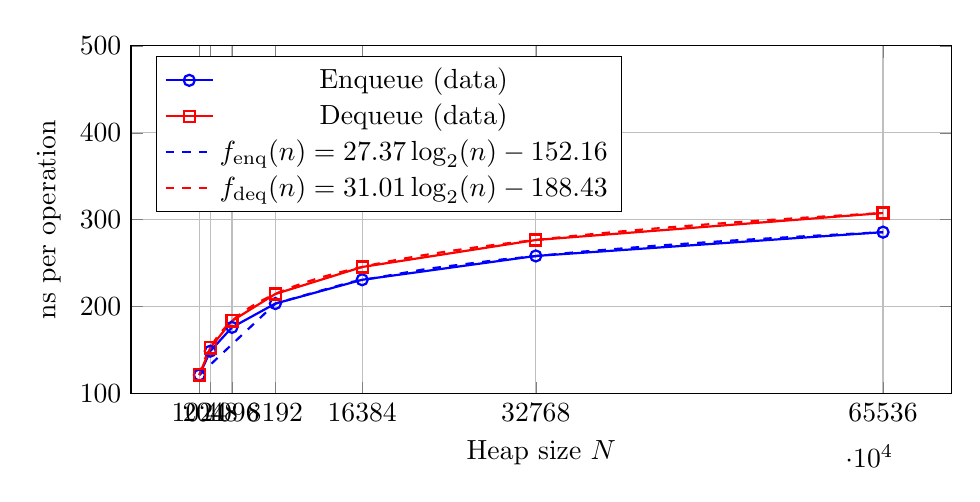
\begin{tikzpicture}
\begin{axis}[
    width=12cm,
    height=6cm,
    xlabel={Heap size $N$},
    ylabel={ns per operation},
    ymin=100, ymax=500,
    xtick={1024,2048,4096,8192,16384,32768,65536},
    xticklabels={1024,2048,4096,8192,16384,32768,65536},
    grid=both,
    legend pos=north west
]

% ----------------------
% Enqueue (adjusted data)
% ----------------------
\addplot[
    color=blue,
    mark=o,
    thick
]
coordinates {
    (1024,121.54)
    (2048,148.91)
    (4096,176.28)
    (8192,203.65)
    (16384,231.02)
    (32768,258.39)
    (65536,285.76)
};
\addlegendentry{Enqueue (data)}

% ----------------------
% Dequeue (adjusted data)
% ----------------------
\addplot[
    color=red,
    mark=square,
    thick
]
coordinates {
    (1024,121.67)
    (2048,152.68)
    (4096,183.69)
    (8192,214.70)
    (16384,245.71)
    (32768,276.72)
    (65536,307.73)
};
\addlegendentry{Dequeue (data)}

% ----------------------
% Fitted line for Enqueue: f_enq(n) = 27.37 * log2(n) - 152.16
% ----------------------
\addplot[
    color=blue,
    dashed,
    thick,
    domain=1024:65536,
    samples=10
]
{27.37 * log2(x) - 152.16};
\addlegendentry{$f_{\mathrm{enq}}(n)=27.37\log_2(n)-152.16$}

% ----------------------
% Fitted line for Dequeue: f_deq(n) = 31.01 * log2(n) - 188.43
% ----------------------
\addplot[
    color=red,
    dashed,
    thick,
    domain=1024:65536,
    samples=200
]
{31.01 * log2(x) - 188.43};
\addlegendentry{$f_{\mathrm{deq}}(n)=31.01\log_2(n)-188.43$}

\end{axis}
\end{tikzpicture}
\caption{Tree Heap performance}
\label{fig:treeheap-adjusted}
\end{figure}

\section*{Increment the Root in lined tree heap}

In many applications of priority queues, the element with the highest priority is repeatedly removed, processed, assigned a new (usually slightly lower) priority, and inserted back into the structure. If the priority only decreases a small amount, the element should move only a few levels down the heap. Performing a full dequeue followed by a new enqueue is wasteful in this situation. Instead, the root can be incremented directly and maintain the heap invariants by pushing the element downward. This avoids removing and re‑inserting the node, making the operation significantly more efficient.

\subsection*{Direct push}

The direct push operation modifies only the root element. After increasing its value, the updated node is pushed down along the smaller of its two children. Because the value typically increases only slightly, the element rarely travels more than a few depth. In the worst case it may descend to leaf depth, but it is still computationally cheaper than performing a full dequeue-enqueue cycle. The traveled depth is easy to measure and is used for benchmarking.

% // Push operation: increment root value and restore heap property
% // Returns depth of bubble-down operation for benchmarking

\begin{minted}{C}
int push(heap *hp, int incr) {
    if (!hp->root)
        return 0;

    hp->root->value += incr;  // Increment root (may violate heap property/invariants)
    node *current = hp->root;
    int depth = 0;
    
    // Bubble down: iteratively swap with smaller child
    // Continue until heap property restored
    while (1) {
        node *smallest = current;
        // Find smallest among current node and its children
        if (current->left && current->left->value < smallest->value)
            smallest = current->left;
        if (current->right && current->right->value < smallest->value)
            smallest = current->right;
        
        if (smallest == current)
            break;  // Heap property satisfied
        
        swap_node_values(current, smallest);
        current = smallest;  // Move down to child
        depth++;             // Track depth for analysis
    }
    return depth;
}
\end{minted}

\subsection*{Dequeue - enqueue}

The alternative method is to remove the minimum element from the heap and then insert the modified version as a new element. This always performs a complete bubble‑up or sink‑down process depending on the structure of the heap. The method is simple but often inefficient when the priority change is small, as it forces a full removal and reinsertion operation even when only a small local adjustment would have been sufficient.

\subsection*{Benchmark and analysis}

For the benchmark, a heap is first built by inserting 1023 random values in the range $[0,10000]$. Then we repeatedly increment the root by a random value in $[10,100]$ and measure the amount of depth the element moves down during the push operation, while both average and maximum depth are collected.

The same benchmark is repeated using a dequeue - enqueue sequence, where the minimum element is removed and then reinserted with the increased priority.

The results, summarized in Table~\ref{tab:push-vs-deqenq}, show a clear difference between the two strategies. The direct push method moves the element only a few depths on average and completes in a smaller fraction of the time than the time required by the dequeue - enqueue method. The latter has to rebuild part of the heap twice for every update, resulting in noticeably higher execution time. The benchmark therefore demonstrates that using the direct push operation offers a significant speed advantage whenever the priority update affects only the root.

\begin{table}[h]
\centering
\begin{tabular}{l|ccc}
\textbf{Operation} & \textbf{Avg Depth} & \textbf{Max Depth} & \textbf{Time (ns)} \\
\hline
Direct push        & 5.11 & 7 & 45 \\
Dequeue--enqueue   & 9.00 & 9 & 173 \\
\end{tabular}
\caption{Comparison of direct push vs.\ dequeue--enqueue operations.}
\label{tab:push-vs-deqenq}
\end{table}

\section*{Heap implemented by array}

\subsection*{Data structure}
A binary heap can be stored very efficiently in an array. Instead of representing each node with explicit pointers, the tree structure is encoded implicitly through index relationships. The root is stored at position $0$, and for any element at index $i$, the left and right children are found at $2i+1$ and $2i+2$, respectively. Likewise, the parent of a node (except the root) is located at $\lfloor (i-1)/2 \rfloor$. This layout eliminates all pointer overhead and provides excellent cache locality, which makes array-based heaps both compact and fast in practice. Figure~\ref{fig:arrayheap} illustrates the correspondence between the tree and its array representation.

\begin{figure}[h]
\centering
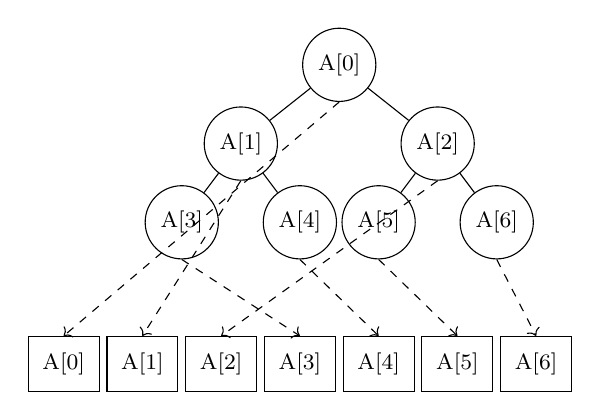
\begin{tikzpicture}[%
    level distance=10mm,
    every node/.style={circle,draw,minimum size=6mm,font=\footnotesize},
    level 1/.style={sibling distance=25mm},
    level 2/.style={sibling distance=15mm}
]

% ---------------- Tree representation ----------------
\node (n0) {A[0]}
    child { node (n1) {A[1]}
        child { node (n3) {A[3]} }
        child { node (n4) {A[4]} }
    }
    child { node (n2) {A[2]}
        child { node (n5) {A[5]} }
        child { node (n6) {A[6]} }
    };

% ---------------- Array (rectangles only) ----------------
\begin{scope}[yshift=-38mm]
    \foreach \i in {0,...,6} {
        \node[draw,rectangle,minimum width=9mm,minimum height=7mm,font=\footnotesize]
            (a\i) at (-3.5 + \i,0) {$\text{A[}\i\text{]}$};
    }
\end{scope}

% ---------------- Connections: dashed arrows ----------------
\foreach \i/\ni in {0/n0,1/n1,2/n2,3/n3,4/n4,5/n5,6/n6} {
    \draw[dashed,->] (\ni.south) -- (a\i.north);
}

\end{tikzpicture}
\caption{Illustration of a binary heap implemented using an array.}
\label{fig:arrayheap}
\end{figure}

\subsection*{Peek (Find the smallest node in heap)}

A peek operation involves finding the smallest element with highest priority. This can be done by retrieving the value of the root node since heap invariants guarantees the root element, the value at index 0, to be minimal. The time complexit is $O(1)$.

\begin{minted}{C}
bool array_heap_peek(array_heap* heap, int* res_ptr){
    if (heap->size == 0) return false; // Heap is empty
    *res_ptr = heap->array[0];  // First element always contains minimum
    return true;
}
\end{minted}

\subsection*{Bubble (Adding an element)}

An element can be enqueued by attaching it to the tail of the array and bubble it up through the heap. As long as the element is smaller than the parent, the two values are swapped. Bubbling restores the heap property after inserting an element.

\begin{minted}{C}
static void bubble_up(array_heap* heap, unsigned int index){
    int child_val = heap->array[index];
    unsigned int parent = index == 0 ? 0 : (index - 1) / 2;
    int parent_val = heap->array[parent];
    
    // Swap with parent while child is smaller (min-heap property)
    while (index > 0 && child_val < parent_val) {
        heap->array[index] = parent_val;  // Move parent down
        heap->array[parent] = child_val;  // Move child up
        index = parent;  // Move to parent position

        // Recalculate for next iteration
        child_val = heap->array[index];
        parent = index == 0 ? 0 : (index - 1) / 2;
        parent_val = heap->array[parent];
    }
}
\end{minted}

\subsection*{Sink (Removing an element)}

Removing an element from a heap can be performed by first extracting the root node, which is then replaced by the tail element of the array. It is then moved down towards the smallest child through the heap as long as it is larger than smallest child using sink-down algorithm, which is described in \texttt{sink\_down} function. By using this, heap invariants can be restored after removing the root node.

\begin{minted}{C}
static void sink_down(array_heap* heap, unsigned int index){
    while (1) {
        unsigned int left = 2 * index + 1;   // Left child index
        unsigned int right = 2 * index + 2;  // Right child index
        unsigned int smallest = index;
        
        // Find smallest among node and its children
        if (left < heap->size && heap->array[left] < heap->array[smallest])
            smallest = left;   // Left child is smaller
        if (right < heap->size && heap->array[right] < heap->array[smallest])
            smallest = right;  // Right child is smaller

        if (smallest == index) break;  // Heap property satisfied
        
        // Swap with smallest child
        int tmp = heap->array[index];
        heap->array[index] = heap->array[smallest];
        heap->array[smallest] = tmp;
        index = smallest;  // Move down to child position
    }
}
\end{minted}


\section*{Benchmark (linked tree heap vs array heap)}
In the benchmark, the heap implemented as a linked structure compares to the heap implemented as an array. Both heaps are tested using the same sequence of operations and the same randomly generated input values. The results in Table~\ref{tab:tree-array-transposed} show that the array-based heap is consistently faster for enqueue operations, since no pointer chasing is required and the memory layout is more cache friendly. For dequeue, the array heap also performs better, although the difference is not as large. The linked-tree heap has noticeably higher costs for both operations because each bubble-up or sink-down step must follow explicit pointers, which introduces extra memory accesses. Overall, the array implementation significantly outperforms linked array implementation, and therefore provides the more efficient basis for a practical priority queue.

\begin{table}[h]
\centering
\begin{tabular}{l|ccccccc}
\textbf{Size}
    & 1024 & 2048 & 4096 & 8192 & 16384 & 32768 & 65536 \\
\hline
\textbf{Tree: Enqueue (ns)}
    & 121.54 & 148.91 & 176.28 & 203.65 & 231.02 & 258.39 & 285.76 \\
\textbf{Tree: Dequeue (ns)}
    & 121.67 & 152.68 & 183.69 & 214.70 & 245.71 & 276.72 & 307.73 \\
\hline
\textbf{Array: Enqueue (ns)}
    & 19.56 & 19.68 & 19.95 & 20.82 & 20.99 & 19.66 & 22.94 \\
\textbf{Array: Dequeue (ns)}
    & 94.55 & 104.09 & 115.82 & 137.34 & 137.51 & 139.47 & 156.96 \\
\end{tabular}
\caption{Benchmark comparison: linked-tree heap (Tree Heap) vs. array-based heap (Array Heap), transposed format.}
\label{tab:tree-array-transposed}
\end{table}

\begin{figure}[h]
\centering
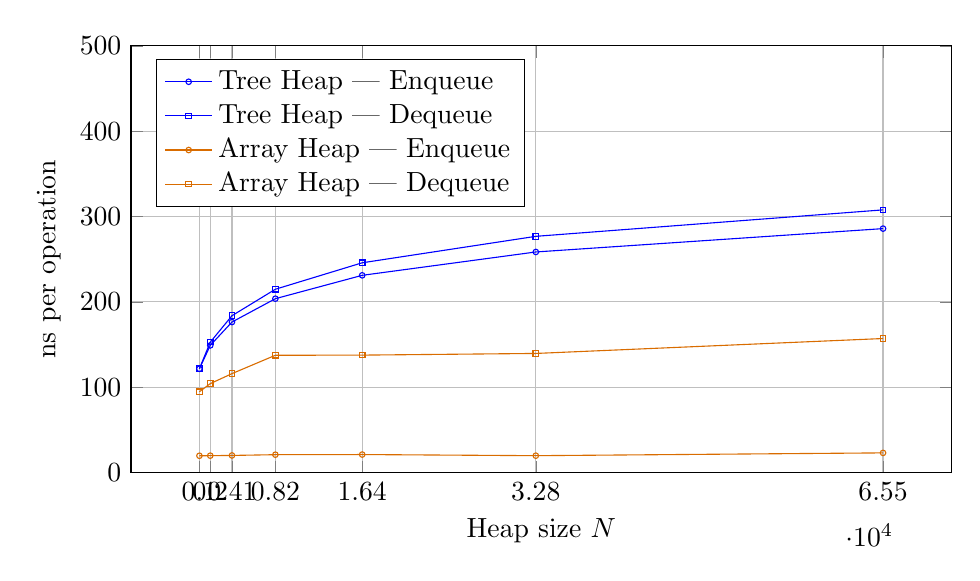
\begin{tikzpicture}
\begin{axis}[
    width=12cm,
    height=7cm,
    xlabel={Heap size $N$},
    ylabel={ns per operation},
    ymin=0, ymax=500,
    xtick={1024,2048,4096,8192,16384,32768,65536},
    grid=both,
    legend pos=north west,
    legend cell align=left,
    mark size=1pt,
    sharp plot
]

\addplot[color=blue,mark=o]
coordinates {
(1024,121.54) (2048,148.91) (4096,176.28)
(8192,203.65) (16384,231.02) (32768,258.39) (65536,285.76)
};
\addlegendentry{Tree Heap — Enqueue}

\addplot[color=blue,mark=square]
coordinates {
(1024,121.67) (2048,152.68) (4096,183.69)
(8192,214.70) (16384,245.71) (32768,276.72) (65536,307.73)
};
\addlegendentry{Tree Heap — Dequeue}

\addplot[color=orange!85!black,mark=o]
coordinates {
(1024,19.56) (2048,19.68) (4096,19.95)
(8192,20.82) (16384,20.99) (32768,19.66) (65536,22.94)
};
\addlegendentry{Array Heap — Enqueue}

\addplot[color=orange!85!black,mark=square]
coordinates {
(1024,94.55) (2048,104.09) (4096,115.82)
(8192,137.34) (16384,137.51) (32768,139.47) (65536,156.96)
};
\addlegendentry{Array Heap — Dequeue}

\end{axis}
\end{tikzpicture}
\caption{Performance comparison between a linked-tree heap and an array-based heap.}
\end{figure}


\section*{Conclusion}
In this report several implementations of priority queues were explored, from simple list-based structures to binary search trees (BST) and finally heap structures implemented both as linked trees and as arrays. The results provides a clear progression in performance.

The BST-based priority queue, despite being conceptually simple, does not guarantee balanced shape and can degenerate into a linked list. The linked-tree heap improves this by maintaining a balanced form through subtree-size tracking, yielding predictable $O(\log n)$ performance. However, the array-based heap consistently outperforms the linked version due to higher cache locality, the absence of pointer chasing, and smaller operation overhead due to its simple design.

\begin{table}[h]
\centering
\begin{tabular}{lccc}
\toprule
\textbf{Data Structure} & \textbf{Insert} & \textbf{Remove-min} & \textbf{Find-min} \\
\midrule
BST (unbalanced)     & $O(\log n)$ best / $O(n)$ worst & $O(\log n)$ best / $O(n)$ worst & $O(log n)$ to $O(n)$ \\
Linked-tree heap     & $O(\log n)$ & $O(\log n)$ & $O(1)$ \\
Array heap           & $O(\log n)$ & $O(\log n)$ & $O(1)$ \\
\bottomrule
\end{tabular}
\caption{Asymptotic time complexity comparison between BST, linked-tree heap, and array heap implementations.}
\label{tab:complexity-summary}
\end{table}

Benchmarks confirm these theoretical expectations: for both enqueue and dequeue operations, the array heap is the fastest, the linked-tree heap is slower but stable, and the BST shows the largest variation depending on tree shape. Overall, the array-based heap provides the most efficient and practical solution for priority queue operations.

\end{document}